\documentclass[light]{theme-beamer}

\usepackage[english]{babel}
\usepackage{amsmath, amssymb, bm}
\usepackage{booktabs, tabularx, array}
\usepackage{graphicx}
\usepackage{tikz}
\usetikzlibrary{arrows.meta}
% stage colours of the plots (src/p1_profiling/plots/style.py), used by the workload figure
\definecolor{visc}{HTML}{2A78D6}
\definecolor{conc}{HTML}{EB6834}
\definecolor{prec}{HTML}{1BAF7A}
\definecolor{denc}{HTML}{EDA100}

% Outline
\AtBeginSection[]
{
\begin{frame}[plain,noframenumbering]
\frametitle{Outline}
\begin{columns}[T]
    \begin{column}{0.01\textwidth}
    \end{column}
    \begin{column}{0.95\textwidth}
        \tableofcontents[currentsection, hideothersubsections]
    \end{column}
\end{columns}
\end{frame}
}

\graphicspath{{../figures/}{../figures/plots/}{../figures/polimi/}{../figures/papers/}{shared/}{./}}

% Project Metadata
\title[Edge NPU for VLAs]{Workload-Driven Exploration of Edge NPU Architectures for Vision-Language-Action Models}
\subtitle{01 --- SmolVLA End-to-End Profiling on PyTorchSim}
\author{Alessandro Ghiotto}
\institute{Politecnico di Milano --- MSc in High Performance Computing Engineering}
\date{October 2026}
\setdepartment{}

\begin{document}

\begin{frame}[plain]
    \titlepage
\end{frame}

% =================================================
\section{Setup}
% =================================================
\subsection{Goal}
\begin{frame}{Goal of Part 1}
    \begin{itemize}
        \item \textbf{Question}: where does the time of one SmolVLA inference go on an NPU?
        \item \textbf{And}: how does the split change from a big NPU to an edge one?
        \vspace{0.8em}
        \item \textbf{Tools}:
        \begin{itemize}
            \item \textit{PyTorchSim}: end-to-end, cycle-level simulation of the whole model.
            \item \textit{Roofline}: what a perfectly tiled NPU could do.
            \item \textit{SCALE-Sim v3}: only a cross-check of single GEMMs (DSE comes in part 2).
        \end{itemize}
        \vspace{0.8em}
        \item One \textbf{action chunk} (50 actions), fp32, batch 1:
        \[
            T_\text{chunk} = 3\,(T_\text{vision} + T_\text{connector}) + T_\text{prefix} + 10\,T_\text{denoise}
        \]
    \end{itemize}
\end{frame}

\subsection{SmolVLA as a workload}
\begin{frame}{SmolVLA as a Workload}
    \begin{figure}
        \centering
        \resizebox{0.9\textwidth}{!}{% !TEX root = ../main.tex
% SmolVLA as a workload: block height is proportional to the number of tokens of each stage.
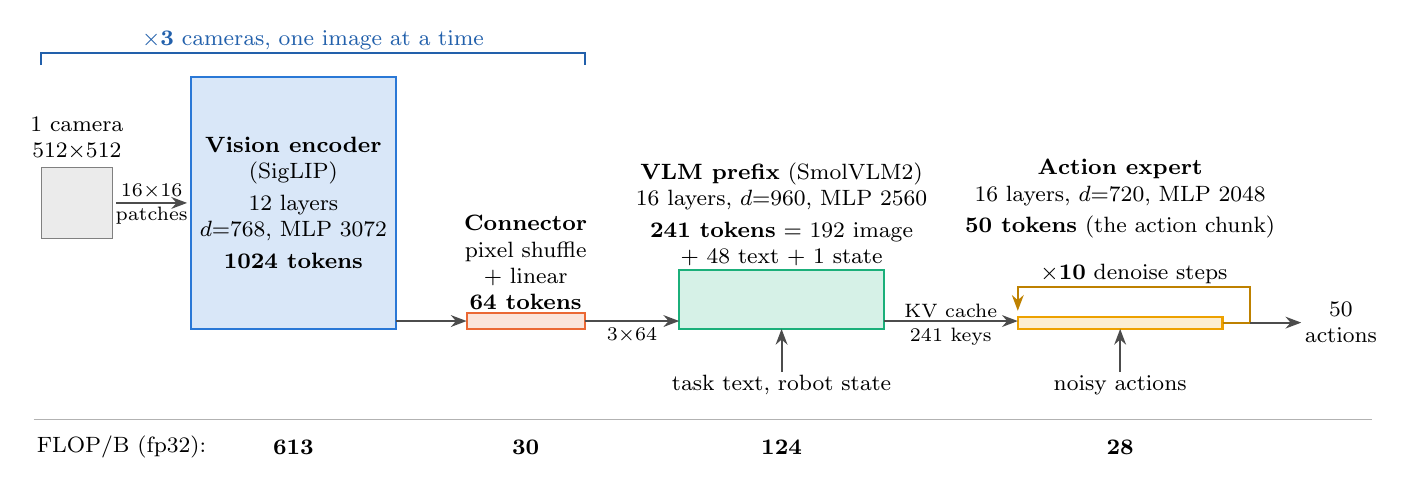
\begin{tikzpicture}[
    font=\footnotesize,
    blk/.style={draw=#1, fill=#1!18, line width=0.8pt},
    lab/.style={align=center, inner sep=1pt},
    arr/.style={-{Stealth[length=2mm]}, line width=0.7pt, draw=black!70},
  ]
  \def\h{3.2/1024}   % cm per token
  % ---- input: one camera image at a time (3 cameras -> vision and connector run 3 times)
  \draw[fill=black!8, draw=black!50] (0, 1.15) rectangle ++(0.9, 0.9);
  \node[lab, above] at (0.45, 2.1) {1 camera\\$512{\times}512$};
  % ---- vision encoder: 1024 tokens
  \draw[blk=visc] (1.9, 0) rectangle (4.5, 3.2);
  \node[lab] at (3.2, 1.6) {\textbf{Vision encoder}\\(SigLIP)\\[2pt]12 layers\\$d{=}768$, MLP 3072\\[2pt]\textbf{1024 tokens}};
  \draw[visc!80!black, line width=0.7pt] (0, 3.35) -- (0, 3.5) -- node[lab, above] {\textbf{$\times$3} cameras, one image at a time} (6.9, 3.5) -- (6.9, 3.35);
  \draw[arr] (0.95, 1.6) -- node[lab, above] {\scriptsize $16{\times}16$} node[lab, below] {\scriptsize patches} (1.85, 1.6);
  % ---- connector: 64 tokens per camera
  \draw[blk=conc] (5.4, 0) rectangle (6.9, 64*\h);
  \node[lab, above] at (6.15, 64*\h) {\textbf{Connector}\\pixel shuffle\\+ linear\\\textbf{64 tokens}};
  \draw[arr] (4.5, 0.1) -- (5.4, 0.1);
  % ---- prefix: 192 image + 48 text + 1 state = 241 tokens
  \draw[blk=prec] (8.1, 0) rectangle (10.7, 241*\h);
  \node[lab, above] at (9.4, 241*\h) {\textbf{VLM prefix} (SmolVLM2)\\16 layers, $d{=}960$, MLP 2560\\[2pt]\textbf{241 tokens} = 192 image\\+ 48 text + 1 state};
  \draw[arr] (6.9, 0.1) -- node[lab, below=1pt] {\scriptsize $3{\times}64$} (8.1, 0.1);
  \node[lab, anchor=north] (txt) at (9.4, -0.55) {task text, robot state};
  \draw[arr] (txt.north) -- (9.4, 0);
  % ---- action expert: 50 tokens, 10 steps
  \draw[blk=denc] (12.4, 0) rectangle (15.0, 50*\h);
  \node[lab, above] at (13.7, 50*\h+0.95) {\textbf{Action expert}\\16 layers, $d{=}720$, MLP 2048\\[2pt]\textbf{50 tokens} (the action chunk)};
  \draw[arr] (10.7, 0.1) -- node[lab, above] {\scriptsize KV cache} node[lab, below=1pt] {\scriptsize 241 keys} (12.4, 0.1);
  \draw[arr, draw=denc!80!black] (15.0, 0.08) -- ++(0.35, 0) -- ++(0, 0.45) -- node[lab, above] {\textbf{$\times$10} denoise steps} ++(-2.95, 0) -- ++(0, -0.3);
  \node[lab, anchor=north] (noise) at (13.7, -0.55) {noisy actions};
  \draw[arr] (noise.north) -- (13.7, 0);
  \draw[arr] (15.35, 0.08) -- (16.0, 0.08) node[lab, right] {50\\actions};
  % ---- arithmetic intensity row
  \draw[black!30] (-0.1, -1.15) -- (16.9, -1.15);
  \node[lab, anchor=west] at (-0.1, -1.5) {FLOP/B (fp32):};
  \node[lab] at (3.2, -1.5) {\textbf{613}};
  \node[lab] at (6.15, -1.5) {\textbf{30}};
  \node[lab] at (9.4, -1.5) {\textbf{124}};
  \node[lab] at (13.7, -1.5) {\textbf{28}};
\end{tikzpicture}
}
    \end{figure}
    \vspace{-0.5em}
    \begin{itemize}
        \item Transformers everywhere: what changes is the \textbf{number of tokens} per weight.
        \item Linear layer $Y_{M\times N} = X_{M\times K}\,W_{K\times N}$ ($M$ tokens, $K$ in / $N$ out features): $2MNK$ FLOPs for $4NK$ weight bytes $\Rightarrow$ \textbf{FLOP/B $\approx M/2$}.
        \item Vision is \textit{compute-bound}, the action expert is \textit{memory-bound} (${\approx}400$~MB of weights per step).
    \end{itemize}
\end{frame}

\subsection{PyTorchSim}
\begin{frame}{PyTorchSim}
    \begin{figure}
        \centering
        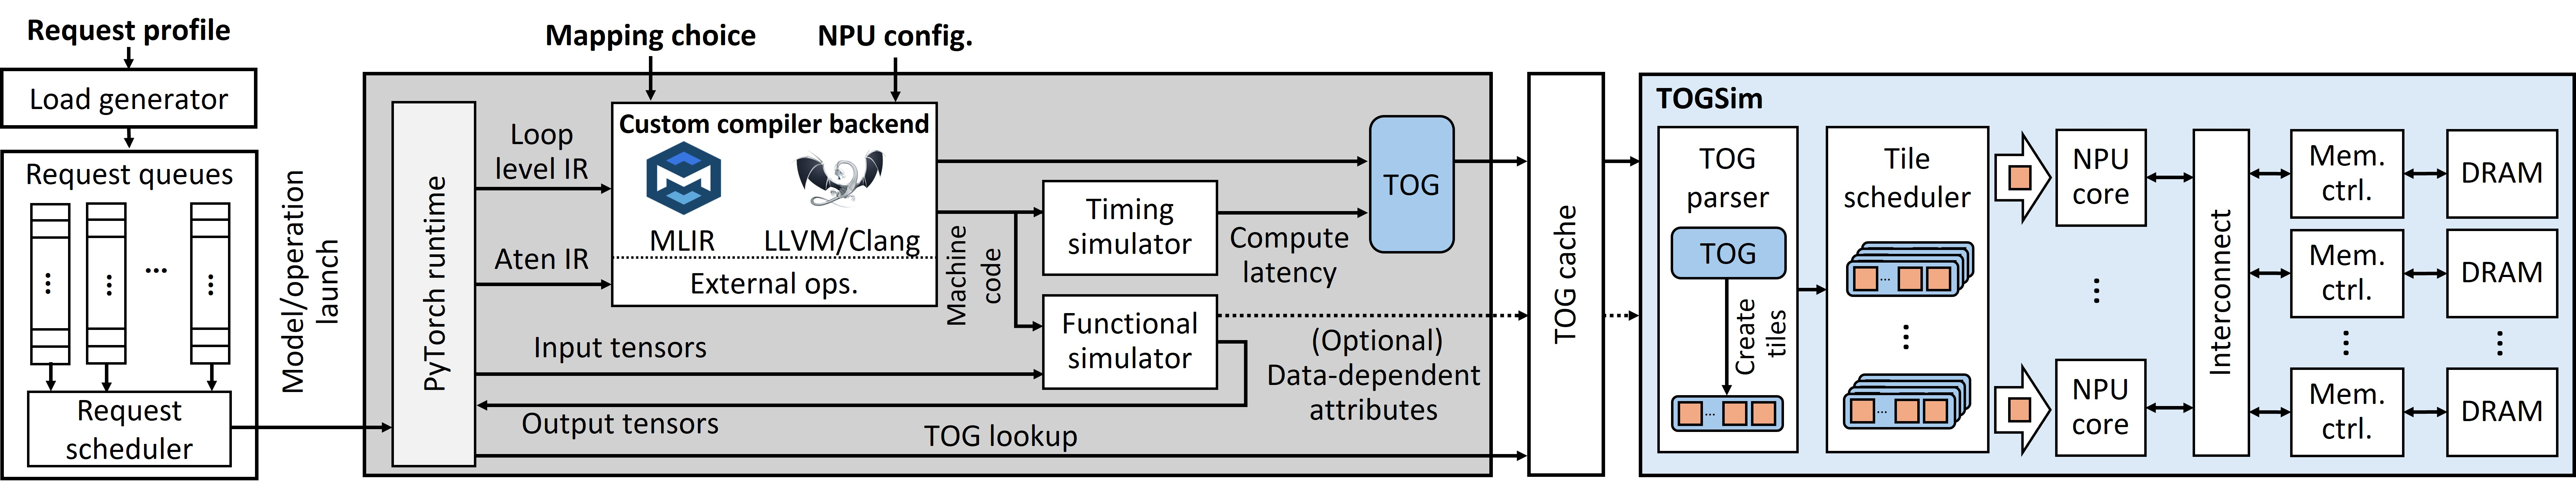
\includegraphics[width=\textwidth]{6.1-pytorchsim-overview.jpg}
        \caption{PyTorchSim overview}
    \end{figure}
    \begin{itemize}
        \item \textbf{Compiler}: \texttt{torch.compile} $\to$ MLIR templates / vector code $\to$ tile-operation graph (TOG).
        \item \textbf{TOGSim}: replays the TOGs on NPU cores; DRAM cycle-accurate (Ramulator 2).
        \item \textbf{Mapping}: heuristic tile sizes that fill the scratchpad.
    \end{itemize}
\end{frame}

\begin{frame}{Simulated NPUs}
    \begin{columns}[c]
        \begin{column}{0.38\textwidth}
            \begin{figure}
                \centering
                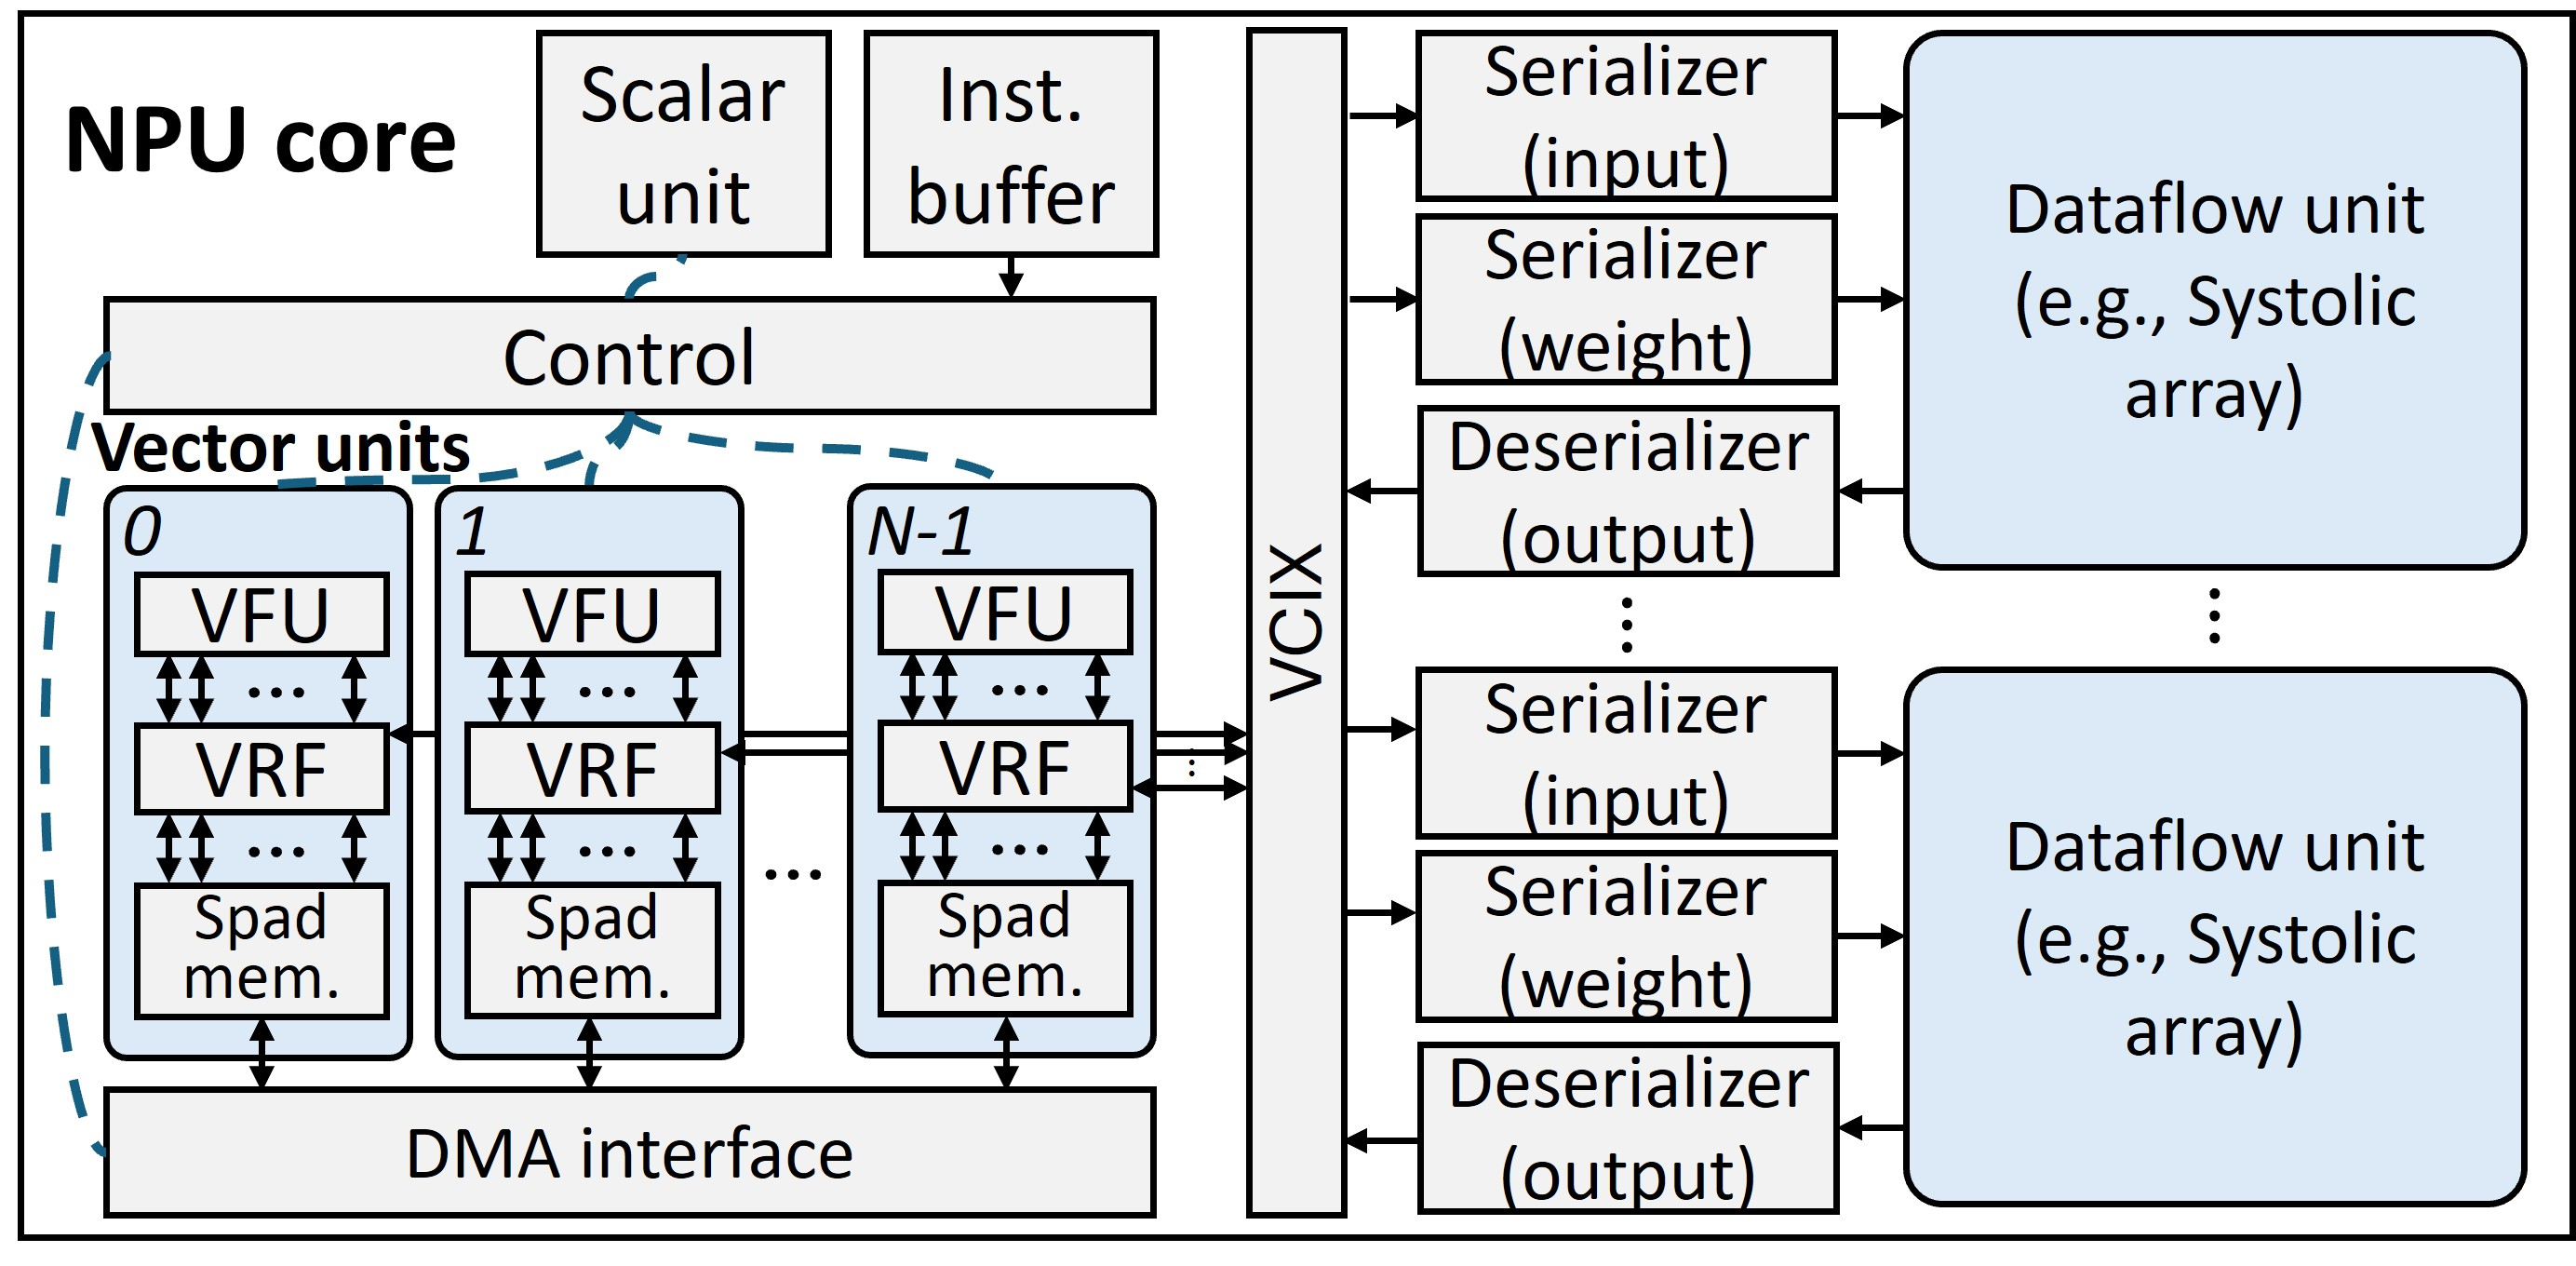
\includegraphics[width=\textwidth]{6.2-pytorchsim-npu-core.jpg}
                \caption{NPU core: $\ell$ vector lanes, $\ell\times\ell$ systolic array}
            \end{figure}
        \end{column}
        \begin{column}{0.62\textwidth}
            \footnotesize
            \setlength{\tabcolsep}{4pt}
            \begin{tabular}{l r r r r}
                \toprule
                NPU & TFLOP/s & Spad & GB/s & Ridge \\
                \midrule
                Big: $2\times128^2$, HBM2 & 61.6 & 16 MB & 481 & 128 \\
                Edge $64\times64$ & 8.2 & 4 MB & 51.2 & 160 \\
                Edge $32\times32$ & 2.0 & 2 MB & 51.2 & 40 \\
                BW sweep $64\times64$ & 8.2 & 4 MB & 12.8--205 & 640--40 \\
                Array sweep & 2.0--32.8 & 4 MB & 51.2 & 40--640 \\
                \bottomrule
            \end{tabular}
            \vspace{1em}
            \begin{itemize}
                \item \textbf{Ridge point} = peak / bandwidth (FLOP/B).
            \end{itemize}
        \end{column}
    \end{columns}
\end{frame}

\subsection{Method}
\begin{frame}{Method: Roofline and Attribution}
    \begin{itemize}
        \item \textbf{Roofline ideal} per stage ($F$ FLOPs, $Q$ compulsory bytes):
        \[
            T_\text{ideal} = \max\left(\frac{F}{P},\ \frac{Q}{B}\right)
        \]
        \item \textbf{Instruction-level replay} of every run (cycle-identical):
        \begin{itemize}
            \item \textit{Time}: array busy / vector unit only / waiting on DRAM.
            \item \textit{Traffic}: compulsory / kernel round trips / weight and activation re-reads.
        \end{itemize}
        \item \textbf{Forced tiling}: traffic-minimising GEMM tiles, to separate the compiler from the hardware.
    \end{itemize}
\end{frame}

% =================================================
\section{Results}
% =================================================
\subsection{Big and edge NPUs}
\begin{frame}{Big NPU: Single Layers}
    \begin{columns}[c]
        \begin{column}{0.4\textwidth}
            \begin{itemize}
                \item Chunk: \textbf{105 ms}.
                \item Vision 60\%, prefix 8\%, denoise 32\%.
                \item Layers far below their roofline bound.
                \item Arrays busy only 15\% of the time.
            \end{itemize}
        \end{column}
        \begin{column}{0.6\textwidth}
            \begin{figure}
                \centering
                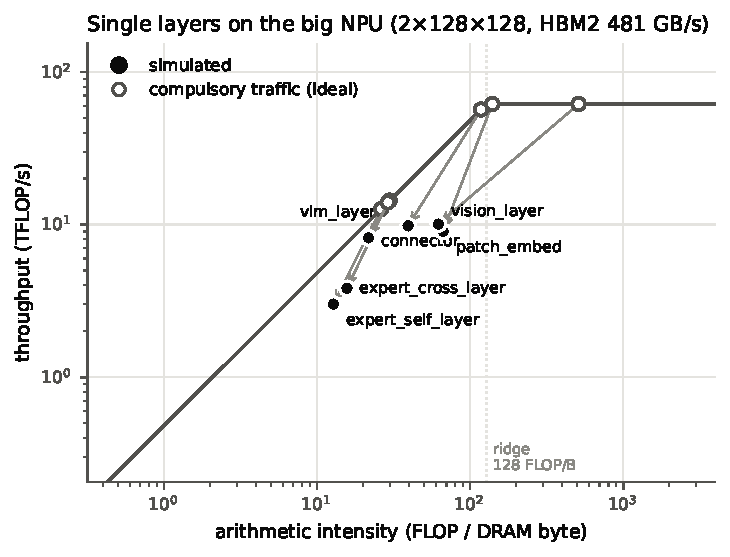
\includegraphics[width=\textwidth]{p1/roofline_layers.pdf}
            \end{figure}
        \end{column}
    \end{columns}
\end{frame}

\begin{frame}{Edge NPUs: Where the Chunk Goes}
    \begin{itemize}
        \item Chunk: \textbf{689 ms} on $64\times64$, \textbf{1030 ms} on $32\times32$.
        \item Compute and bandwidth shrink together: what matters is the \textbf{ridge point}.
    \end{itemize}
    \begin{figure}
        \centering
        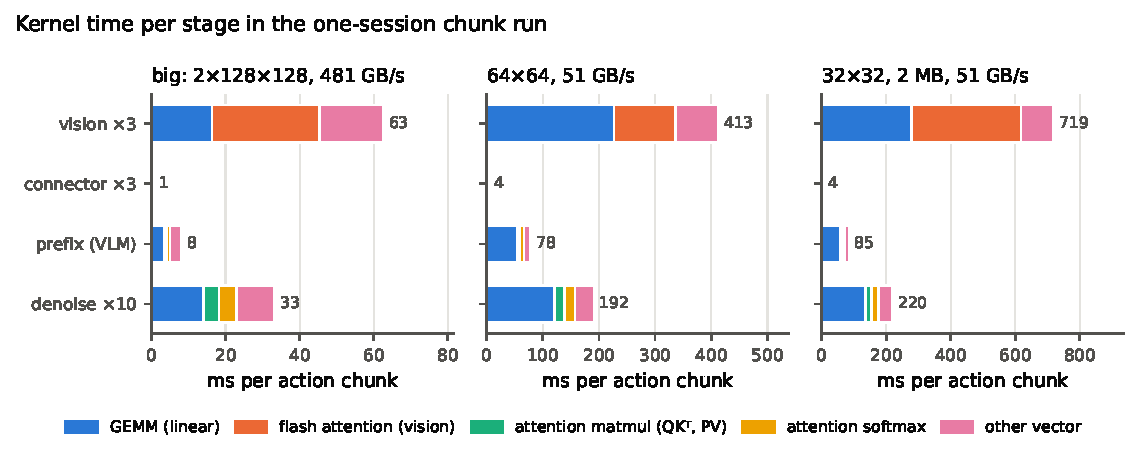
\includegraphics[width=0.95\textwidth]{p1/kernel_classes.pdf}
    \end{figure}
\end{frame}

\begin{frame}{Edge $64\times64$: Kernel Timeline}
    \begin{itemize}
        \item Strictly sequential: $3\times$ vision + connector, prefix, $10\times$ denoise.
    \end{itemize}
    \begin{figure}
        \centering
        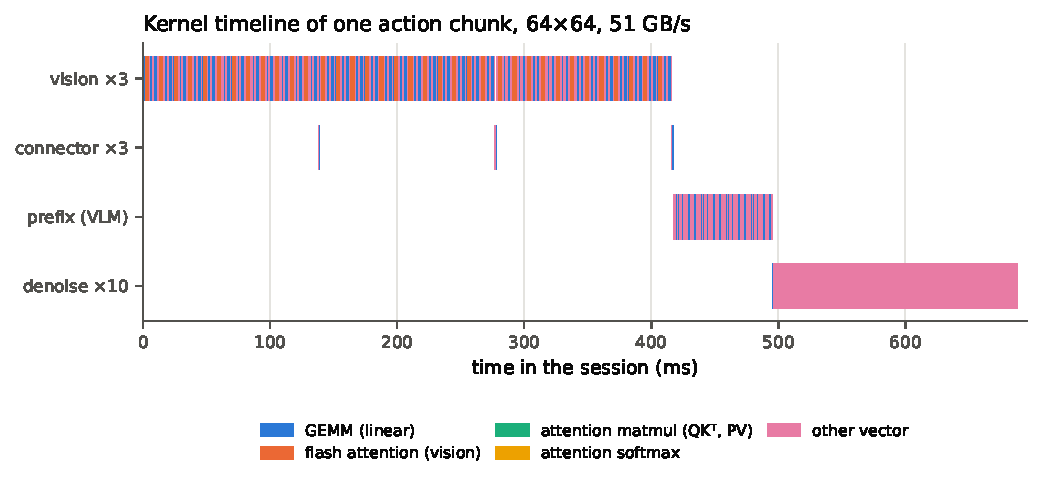
\includegraphics[width=0.9\textwidth]{p1/kernel_timeline.pdf}
    \end{figure}
\end{frame}

\subsection{Sweeps}
\begin{frame}{Bandwidth Sweep ($64\times64$)}
    \begin{itemize}
        \item Simulated: bandwidth-bound end to end (half the bandwidth, twice the time); vision dominates at every bandwidth.
        \item Ideal: the action expert \textbf{takes over} as bandwidth drops.
    \end{itemize}
    \begin{figure}
        \centering
        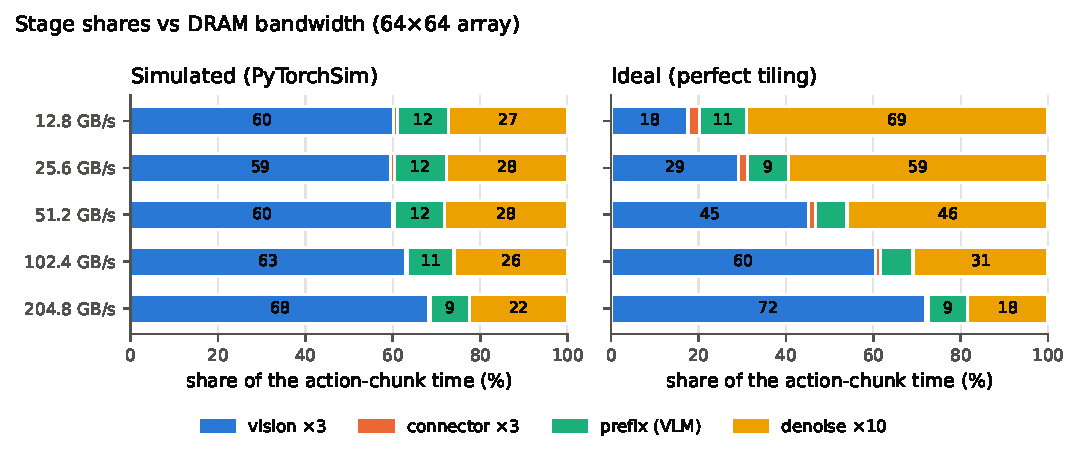
\includegraphics[width=0.85\textwidth]{p1/bandwidth_shares.pdf}
    \end{figure}
\end{frame}

\begin{frame}{Array-Size Sweep (51.2 GB/s)}
    \begin{itemize}
        \item Diminishing returns from $32\times32$ to $128\times128$.
        \item Prefix and denoise stay pinned at the DRAM limit.
    \end{itemize}
    \begin{figure}
        \centering
        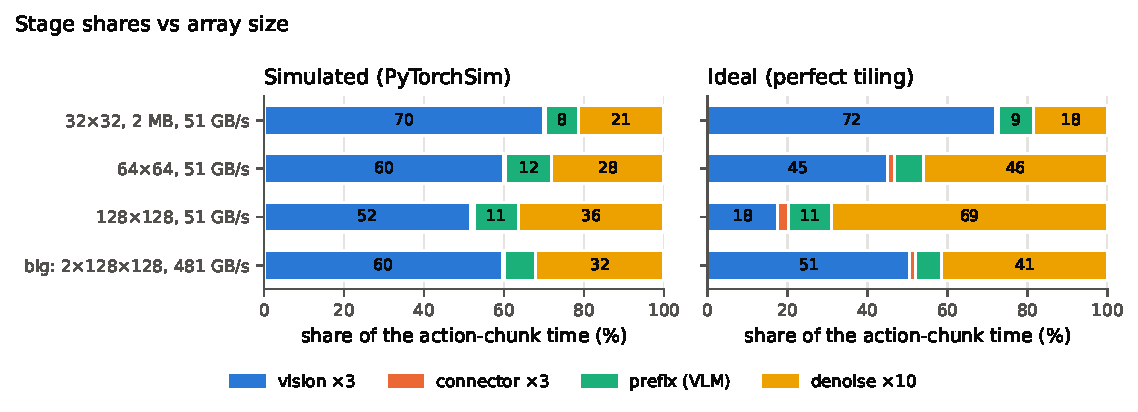
\includegraphics[width=0.85\textwidth]{p1/array_shares.pdf}
    \end{figure}
\end{frame}

\subsection{Where the time and the traffic go}
\begin{frame}{Roofline per Stage}
    \begin{itemize}
        \item Vision: compute-bound on paper, but moves \textbf{10--17$\times$} its compulsory traffic.
        \item Prefix 3--7$\times$, denoise ${\approx}2\times$.
    \end{itemize}
    \begin{figure}
        \centering
        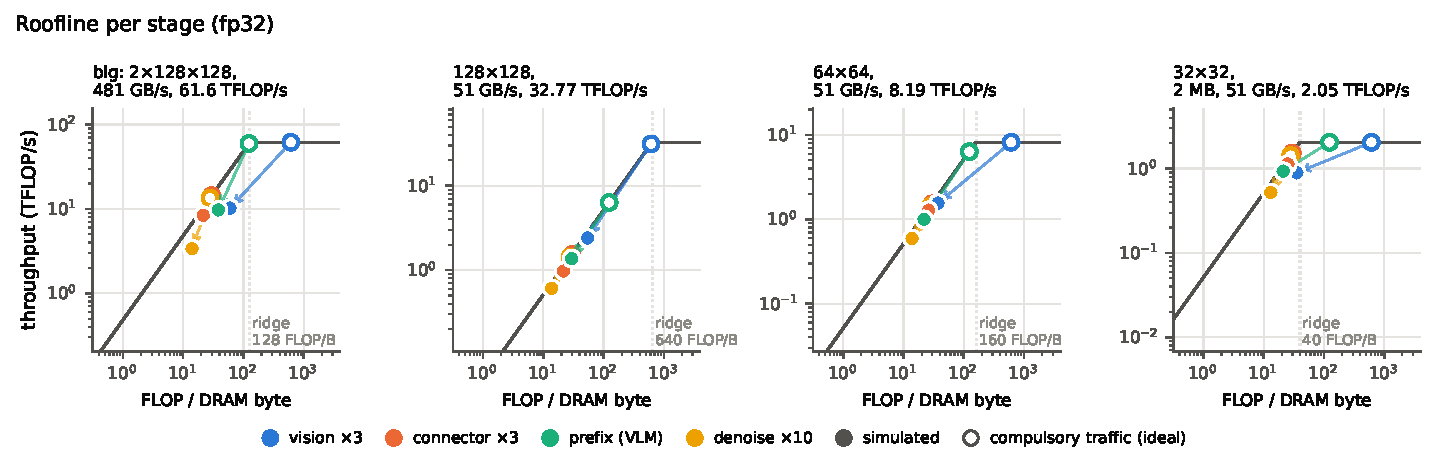
\includegraphics[width=\textwidth]{p1/roofline_stages.pdf}
    \end{figure}
\end{frame}

\begin{frame}{Where the Time Goes}
    \begin{itemize}
        \item The \textbf{array is not the bottleneck}: it streams at the ideal rate (up to padding).
        \item Time is lost \textbf{waiting on DRAM} and on the vector unit.
    \end{itemize}
    \begin{figure}
        \centering
        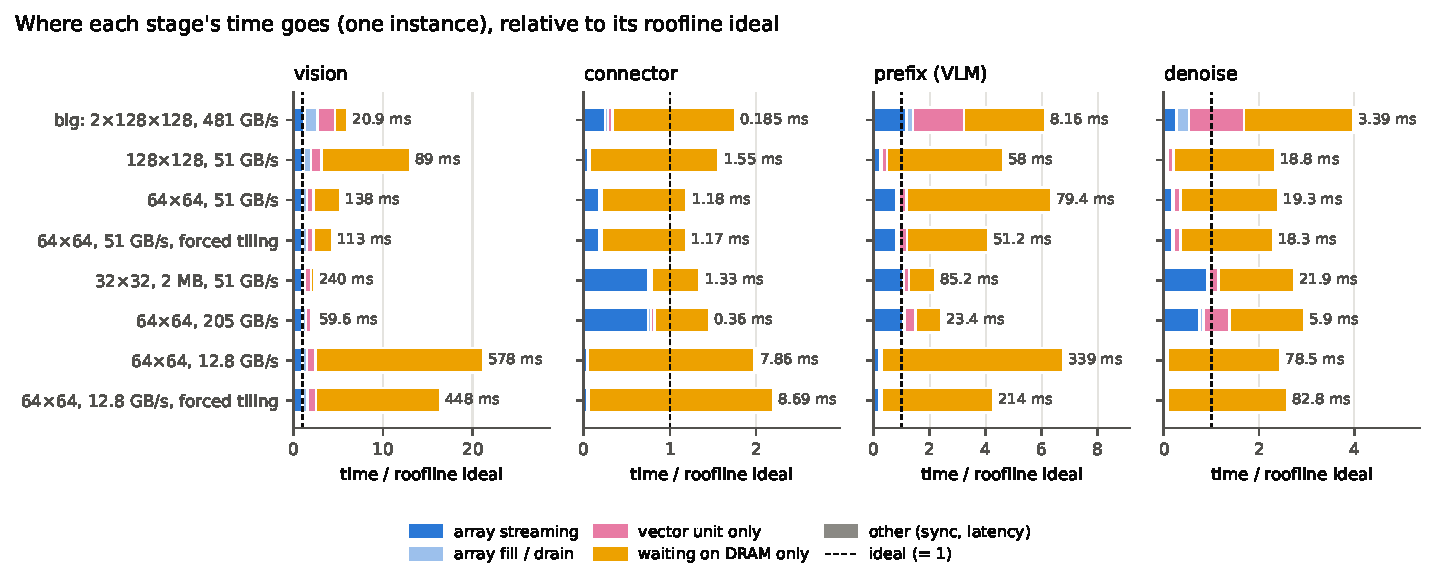
\includegraphics[width=0.92\textwidth]{p1/attribution_time.pdf}
    \end{figure}
\end{frame}

\begin{frame}{Where the Traffic Comes From}
    \begin{itemize}
        \item \textbf{Vision}: weight re-reads, flash-attention K/V re-reads, kernel round trips.
        \item \textbf{Denoise}: no tiling waste; extra traffic = round trips between small kernels.
    \end{itemize}
    \begin{figure}
        \centering
        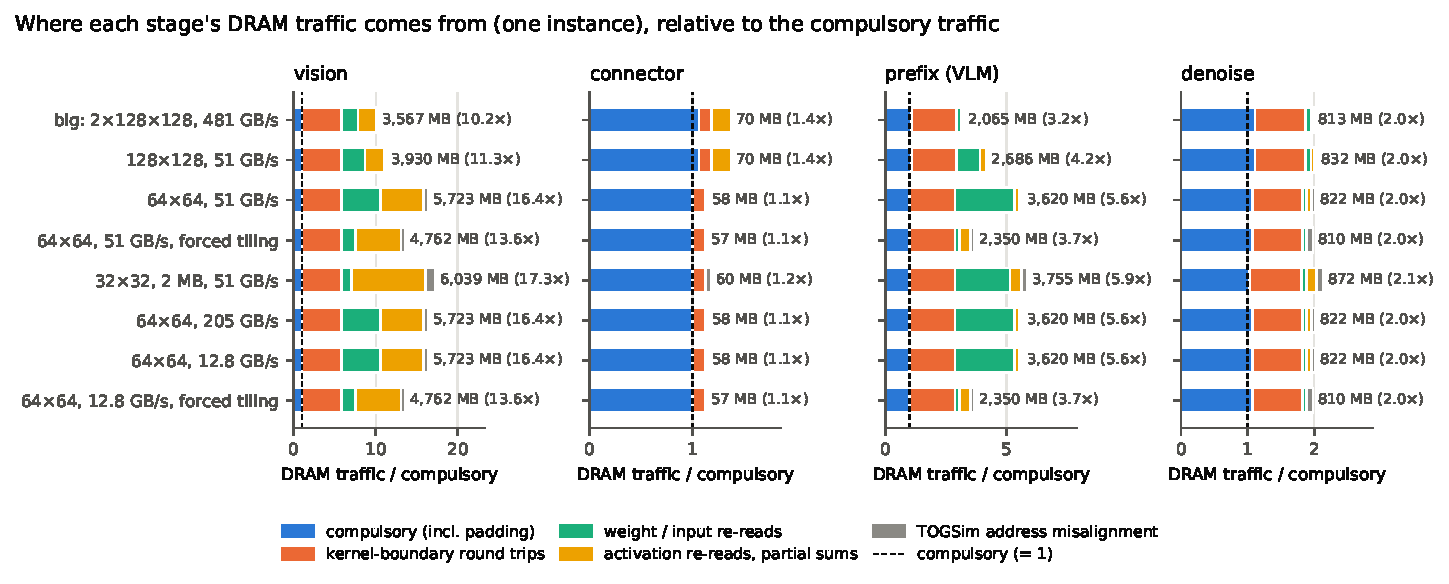
\includegraphics[width=0.92\textwidth]{p1/attribution_traffic.pdf}
    \end{figure}
\end{frame}

\begin{frame}{Does the Action Expert Take Over?}
    \begin{itemize}
        \item Forced tiling: helps prefix and vision, barely denoise.
        \item No round trips (estimate): denoise gets close to its ideal.
        \item Vision still far above compulsory traffic: 4 MB scratchpad, flash-attention tiling.
    \end{itemize}
    \begin{figure}
        \centering
        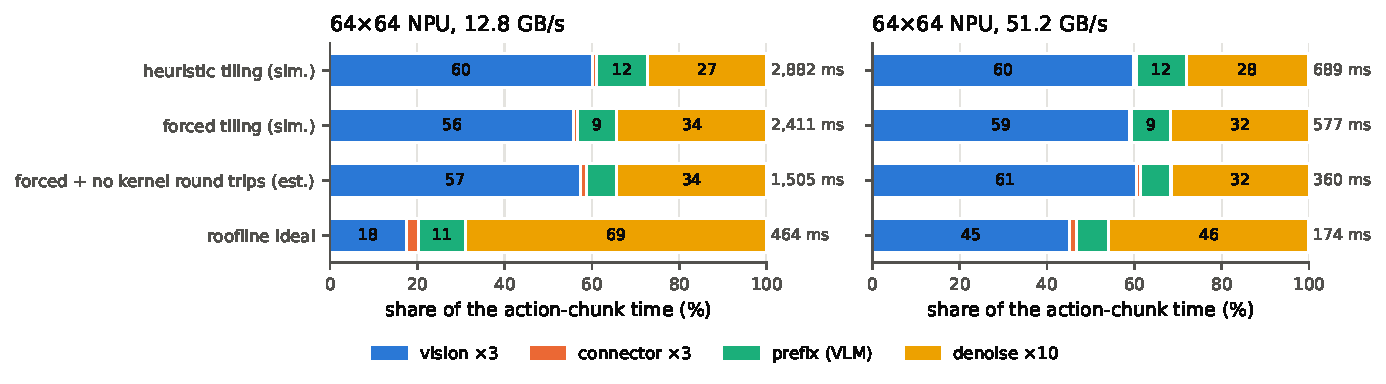
\includegraphics[width=\textwidth]{p1/scenarios.pdf}
    \end{figure}
\end{frame}

\subsection{How the stages respond}
\begin{frame}{How the Stages Respond to the Hardware (1/2)}
    \begin{center}
    \small
    \begin{tabular}{l r r r l}
        \toprule
        Stage (one instance) & GFLOP & Compulsory MB & FLOP/B & Activations \\
        \midrule
        Vision & 214 & 349 & 613 & 3 MB (MLP 12.6 MB) \\
        Connector & 1.5 & 51 & 30 & 3 MB \\
        Prefix & 79 & 641 & 124 & 0.9 MB (MLP 2.5 MB) \\
        Denoise step & 11.3 & 410 & 28 & 0.14 MB (MLP 0.41 MB) \\
        \bottomrule
    \end{tabular}
    \end{center}
    \begin{itemize}
        \item \textbf{Bandwidth} shortens every DRAM wait but removes no byte.
        \begin{itemize}
            \item Ideally: only memory-bound stages gain (denoise, connector, prefix above 124 FLOP/B).
            \item Simulated: vision gains too, its extra traffic made it memory-bound.
        \end{itemize}
        \item \textbf{Array size} helps only compute-bound work: vision (and prefix), never denoise.
        \item \textbf{Ridge point} sets the ideal split, not the NPU size: the higher the ridge, the larger the denoise share (ceiling: its share of the compulsory bytes).
    \end{itemize}
\end{frame}

\begin{frame}{How the Stages Respond to the Hardware (2/2)}
    \begin{itemize}
        \item \textbf{Scratchpad}:
        \begin{itemize}
            \item \textit{Vision} needs capacity: best tiles reach its minimum GEMM traffic only at ${\approx}64$ MB.
            \item The 16 MB big NPU still moves $10\times$: heuristic tiles (weights $4\times$), flash template (K/V $8\times$), kernel round trips $\Rightarrow$ the \textbf{mapping matters as much as the size}.
            \item \textit{Action expert}: a bigger scratchpad does not help (working set $< 1$ MB); its cost is ${\approx}400$ MB of weights per step.
        \end{itemize}
        \vspace{0.5em}
        \item \textbf{Fusion} (no kernel round trips): cheap for the expert and the prefix, competes with weight tiles in vision.
        \vspace{0.5em}
        \item \textbf{Precision}: bf16 halves, int8 quarters the expert's weight bytes.
        \vspace{0.8em}
        \item[$\Rightarrow$] \textbf{Vision}: compute, vector unit, on-chip capacity. \quad \textbf{Action expert}: bandwidth, fewer bytes per weight.
    \end{itemize}
\end{frame}

\subsection{SCALE-Sim cross-check}
\begin{frame}{Cross-check with SCALE-Sim}
    \begin{columns}[c]
        \begin{column}{0.4\textwidth}
            \begin{itemize}
                \item Large vision GEMMs: good agreement.
                \item Thin GEMMs (expert, VLM): SCALE-Sim much slower.
                \item Cause: per-fold weight load in SCALE-Sim vs double buffering in PyTorchSim.
            \end{itemize}
        \end{column}
        \begin{column}{0.6\textwidth}
            \begin{figure}
                \centering
                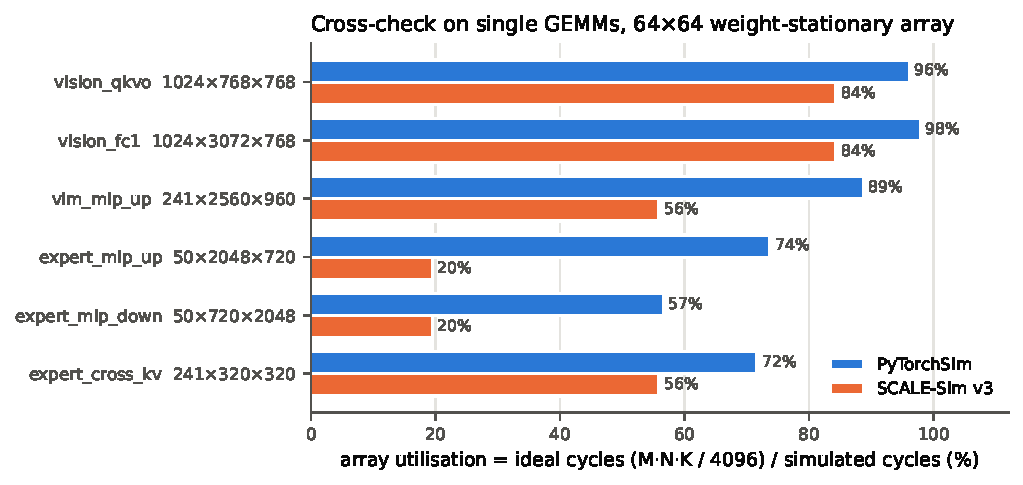
\includegraphics[width=\textwidth]{p1/scalesim_check.pdf}
            \end{figure}
        \end{column}
    \end{columns}
\end{frame}

% =================================================
\section{Takeaways}
% =================================================
\begin{frame}{Takeaways and Next Steps}
    \begin{itemize}
        \item \textbf{Stage balance depends on the compiler as much as on the hardware}.
        \item \textbf{The array is not the bottleneck}: DRAM traffic and vector work are.
        \item \textbf{Opposite demands}: vision $\to$ compute + capacity; action expert $\to$ bandwidth + precision.
        \vspace{0.8em}
        \item \textbf{Part 2}: design-space exploration with SCALE-Sim
        \begin{itemize}
            \item Array size, dataflow, scratchpad size, bandwidth, precision, one at a time.
            \item Towards a heterogeneous edge NPU for VLAs.
        \end{itemize}
    \end{itemize}
\end{frame}

\begin{frame}[plain, noframenumbering]
    \vfill
    \begin{center}
        {\Huge \textbf{Thank you for your attention!}}

        \vspace{1.5em}

        {\Large Questions \& Discussion}
    \end{center}
    \vfill
\end{frame}

\end{document}
